\section{Assignment 1}

\begin{figure}[h]
\centering
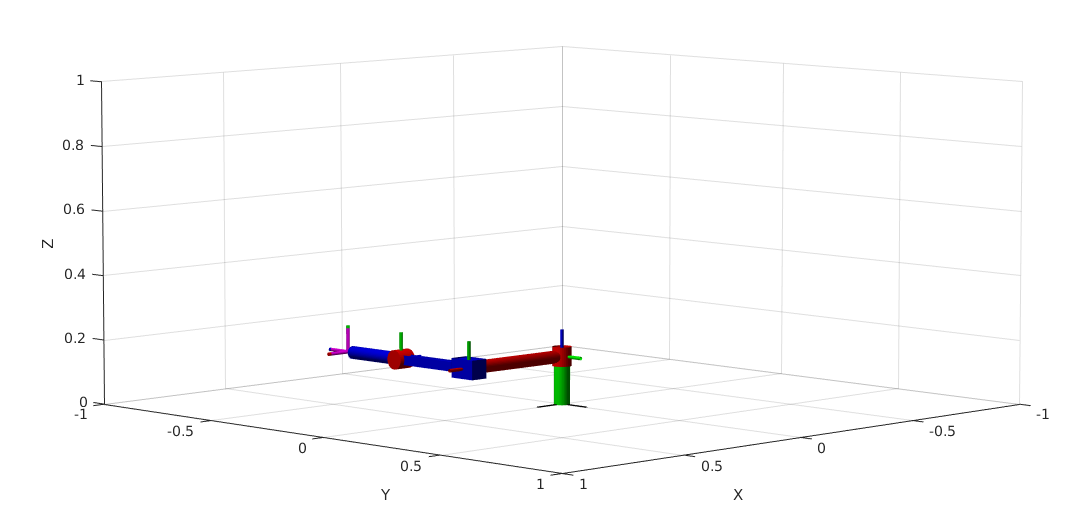
\includegraphics[keepaspectratio,width=0.5\textwidth]{1}
\caption{Visualization of the URDF of the PRP robot in the home configuration ($ q_1=0,q_2=0,\theta_3=0$)}
\end{figure}

\subsection{Denavit-Hartenberg parameters}

First of all, reference frames were assigned to each joint according to the DH convention:

\begin{figure}[h]
\centering
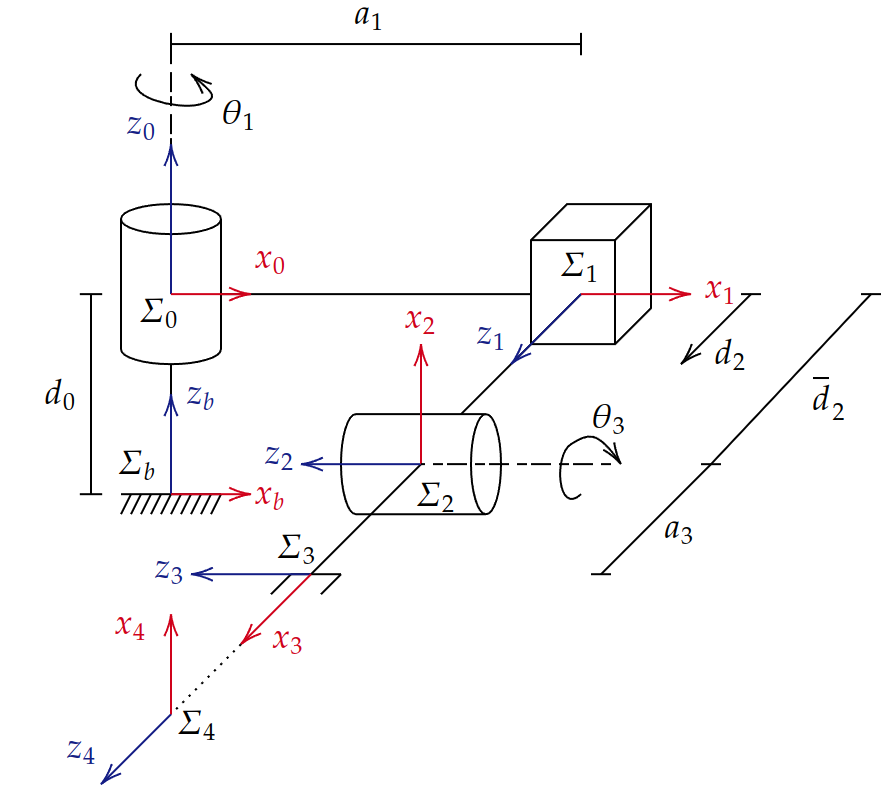
\includegraphics[keepaspectratio,width=0.45\textwidth]{2}
\caption{Reference frames assigned with the DH convention}
\end{figure}

Note that the DH frames do not correspond with the frames of the URDF model.

Then the DH parameter table was populated:

\begin{table}[h]
\centering
\begin{tabular}{c|c|c|c|c}
  & $a_i$ & $\alpha_i$       & $d_i$ & $\theta_i$      \\ \hline
0 & 0 & 0 & $d_0$ & 0\\
1 & $a_1$ & $\frac{\pi}{2}$  & 0     & $q_1 =  \theta_1$ \\
2 & 0     & $-\frac{\pi}{2}$ & $(q_2=d_2)+\overline d_2$ & $\frac{\pi}{2}$ \\
3 & $a_3$     & 0                & 0     & $(q_3=\theta_3)-\frac{\pi}{2}$\\
4 & 0 & $\frac{\pi}{2}$ & 0 & $\frac{\pi}{2}$
\end{tabular}
\end{table}

The first row is the fixed offset in the $z_b$ direction between world and frame $\Sigma_0$, while the last row is the fixed rotation that aligns the $z$ axis of the end-effector to the approach direction.

\newpage

Using the DH parameters, the transformation matrices between the frames were then computed. The transformation matrix between frame $i$ and frame $i-1$ is in the form:

\begin{align*}
T_{i-1}^i=\begin{bmatrix}
\cos(\theta_i)&-\sin(\theta_i)\cos(\alpha_i)&\sin(\theta_i)\sin(\alpha_i)&a_i\cos(\theta_i)\\
\sin(\theta_i)&\cos(\theta_i)\cos(\alpha_i)&-\cos(\theta_i)\sin(\alpha_i)&a_i\sin(\theta_i)\\
0&\sin(\alpha_i)&\cos(\alpha_i)&d_i\\
0&0&0&1
\end{bmatrix}
\end{align*}

The computed transformation matrices are then:
\begin{align*}
T_b^0&=\begin{bmatrix}
1 & 0 & 0 & 0\\ 0 & 1 & 0 & 0\\ 0 & 0 & 1 & d_0\\0 & 0 &0 &1
\end{bmatrix}
\;\;\;\;\;\;\;\;\;T_0^1=\begin{bmatrix}
C_1&0&S_1&a_1C_1\\
S_1&0&-C_1&a_1S_1\\
0&1&0&0\\
0&0&0&1
\end{bmatrix}\;\;\;\;\;\;\;\;\;
T_1^2=\begin{bmatrix}
0&0&-1&0\\
1&0&0&0\\
0&-1&0&q_2+\overline d_2\\
0&0&0&1
\end{bmatrix}\\T_2^3&=\begin{bmatrix}
C\left(q_3-\frac{\pi}{2}\right)&-S\left(q_3-\frac{\pi}{2}\right)&0&a_3C\left(q_3-\frac{\pi}{2}\right)\\
S\left(q_3-\frac{\pi}{2}\right)&C\left(q_3-\frac{\pi}{2}\right)&0&a_3S\left(q_3-\frac{\pi}{2}\right)\\
0&0&1&0\\
0&0&0&1
\end{bmatrix}=\begin{bmatrix}
S_3&C_3&0&a_3S_3\\-C_3&S_3&0&-a_3C_3\\0&0&1&0\\0&0&0&1
\end{bmatrix}\;\;\;\;\;\;\;\;\; T_3^4 = \begin{bmatrix}
0 & 0 & 1 & 0\\
1 & 0 & 0 & 0\\
0 & 1 & 0 & 0\\
0 & 0 & 0 & 1
\end{bmatrix}
\end{align*}

where $C_i$ and $S_i$ denote respectively $\cos(q_i)$ and $\sin(q_i)$.

\subsection{Direct kinematics}

The direct kinematics of the manipulator are obtained by chaining the above transformation matrices, thus obtaining a global transformation matrix from the end-effector to the base of the manipulator:

\begin{align*}
T_b^4&=T_b^0T_0^1T_1^2T_2^3T_3^4=\underset{T_b^1}{\underbrace{\begin{bmatrix}
C_1&0&S_1&a_1C_1\\
S_1&0&-C_1&a_1S_1\\
0&1&0&d_0\\
0&0&0&1
\end{bmatrix}}}T_1^2T_2^3T_3^4=\underset{T_b^2}{\underbrace{\begin{bmatrix}
0 & -S_1&-C_1&(q_2+\overline d_2)S_1+a_1C_1\\
0 & C_1&-S_1&-(q_2+\overline d_2)C_1+a_1S_1\\
1 & 0 & 0 & d_0\\
0&0&0&1
\end{bmatrix}}}T_2^3T_3^4\\
&=\underset{T_b^3}{\underbrace{\begin{bmatrix}
S_1C_3&-S_1S_3&-C_1&(q_2+\overline d_2)S_1+a_1C_1+a_3S_1C_3\\
-C_1C_3&C_1S_3&-S_1&-(q_2+\overline d_2)C_1+a_1S_1-a_3C_1C_3\\
S_3&C_3&0&d_0+a_3S_3\\
0&0&0&1
\end{bmatrix}}}T_3^4\\
&=\begin{bmatrix}
-S_1S_3 & -C_1 & S_1C_3 & (q_2+\overline d_2)S_1+a_1C_1+a_3S_1C_3\\
C_1S_3 & -S_1 & -C_1C_3 & -(q_2+\overline d_2)C_1+a_1S_1-a_3C_1C_3\\
C_3 & 0 & S_3 &d_0+a_3S_3\\
0&0&0&1 
\end{bmatrix} =\begin{bmatrix}
R_b^{4}&p_{4}\\
\overline 0 & 1
\end{bmatrix}
\end{align*}

\subsection{Inverse kinematics}

From the direct kinematics, the position of the end-effector is given by:

\begin{equation*}
p_{4}=\begin{pmatrix}
p_{4x}\\p_{4y}\\p_{4z}
\end{pmatrix}=\begin{pmatrix}
(q_2+\overline d_2)S_1+a_1C_1+a_3S_1C_3\\
-(q_2+\overline d_2)C_1+a_1S_1-a_3C_1C_3\\
d_0+a_3S_3
\end{pmatrix}
\end{equation*}

Therefore an expression for $q_3$ can immediately be derived:

\begin{equation*}
p_{4z}=d_0+a_3S_3\implies S_3=\frac{p_{4z}-d_0}{a_3}, C_3=\pm\sqrt{1-S_3^2}=\pm\sqrt{\frac{a_3^2-(p_{4z}-d_0)^2}{a_3^2}}\implies q_3^\pm=\atan2(S_3,\pm C_3)
\end{equation*}

$q_2$ is determined by applying summing and squaring to the position of the origin of frame $\Sigma_2$:

\begin{equation*}
p_2 = \begin{pmatrix}
p_{2x}\\p_{2y}\\p_{2z}
\end{pmatrix}=\begin{pmatrix}
(q_2+\overline d_2)S_1+a_1C_1\\
-(q_2+\overline d_2)C_1+a_1S_1\\
d_0
\end{pmatrix}
\end{equation*}
\begin{align*}
p_{2x}^2+p_{2y}^2&=S_1^2(q_2+\overline d_2)^2+a_1^2C_1^2+\cancel{2a_1(q_2+\overline d_2)S_1C_1}+C_1^2(q_2+\overline d_2)^2+a_1^2S_1^2-\cancel{2a_1(q_2+\overline d_2)S_1C_1}=\\
&=(q_2+\overline d_2)^2+a_1^2
\end{align*}

Therefore $q_2$ is given by the solution of the quadratic equation:

\begin{equation*}
q_2^2+2\overline d_2q_2+a_2-p_{2x}^2-p_{2y}^2=0
\end{equation*}

which is:

\begin{equation*}
q_{2,12}=-\frac{\cancel{2}\overline d_2\pm\sqrt{\cancel{4\overline d_2^2}-\cancel{4}(a_1^2+\cancel{\overline d_2}-p_{2x}^2-p_{2y}^2)}}{\cancel{2}}=-\overline d_2\pm\sqrt{p_{2x}^2+p_{2y}^2-a_1^2}
\end{equation*}

To choose the solution, both are computed and the correct one will be the one that satisfies joint limits.

To choose the correct sign for $q_3$, $q_2$ is recomputed by summing and squaring the $x$ and $y$ components of $p_3$:

\begin{align*}
p_{3x}^2+p_{3y}^2&=S_1^2(q_2+\overline d_2)^2+a_1^2C_1^2+a_3^2S_1^2C_3^2+\cancel{2a_1(q_2+\overline d_2)S_1C_1}+2a_3(q_2+\overline d_2)S_1^2C_3+\cancel{2a_1a_3S_1C_1C_3}\\&+C_1^2(q_2+\overline d_2)^2+a_1^2S_1^2+a_3^2C_1^2C_3^2-\cancel{2a_1(q_2+\overline d_2)S_1C_1}+2a_3(q_2+\overline d_2)C_1^2C_3-\cancel{2a_1a_3S_1C_1C_3}=\\
&=(q_2+\overline d_2)^2+a_1^2+a_3^2C_3^2+2a_3(q_2+\overline d_2)C_3
\end{align*}

and therefore:

\begin{equation*}
q_{2,12}= -a_3C_3-\overline d_2\pm\sqrt{p_{4x}^2+p_{4y}^2-a_1^2}
\end{equation*}

By computing the four possible solutions and checking which one is equal to the one obtained previously, it is possible to determine the correct sign for $C_3$ and therefore the correct value for $q_3$.

Finally, $q_1$ is determined by solving the system of equations:

\begin{equation*}
\begin{cases}
p_{2x}=(q_2+\overline d_2)S_1+a_1C_1\\
p_{2y}=-(q_2+\overline d_2)C_1+a_1S_1
\end{cases}
\end{equation*}

in the unknowns $C_1$ and $S_1$. The system yields:

\begin{equation*}
C_1 = \frac{a_1p_{2x}-(q_2+\overline d_2)p_{2y}}{(q_2+\overline d_2)^2+a_1^2}, S_1=\frac{p_{2x}-a_1C_1}{(q_2+\overline d_2)}\implies q_1=\atan2(S_1,C_1)
\end{equation*}

For the orientation $o_4$ of the end-effector, the angles $\alpha,\beta$ and $\gamma$ can be derived by equating the rotation matrix $R_b^4$ to the rotation matrix that expresses a $ZXZ$ Euler angle rotation:

\begin{equation*}
\begin{bmatrix}
-S_1S_3 & -C_1 & S_1C_3\\
C_1S_3 & -S_1 & -C_1C_3\\
C_3 & 0 & S_3
\end{bmatrix}=\begin{bmatrix}
C_\alpha C_\gamma-C_\beta S_\alpha S_\gamma & -C_\alpha S_\gamma-C_\beta C_\gamma S_\alpha & S_\alpha S_\beta\\
S_\alpha C_\gamma+C_\beta C_\alpha S_\gamma & -S_\alpha S_\gamma-C_\beta C_\gamma C_\alpha & -C_\alpha S_\beta\\
S_\beta S_\gamma & C_\gamma S_\beta & C_\beta
\end{bmatrix}
\end{equation*}

\begin{equation*}
\begin{cases}
S_\alpha S_\beta = S_1C_3, -C_\alpha S_\beta = -C_1C_3 \implies S_\alpha=S_1,C_\alpha=C_1&\implies \alpha = q_1\\ 
C_\beta = S_3&\implies \beta = \frac{\pi}{2}-q_3\\
S_\beta S_\gamma = C_3\implies S_\gamma = 1&\implies \gamma = \frac{\pi}{2}
\end{cases}
\implies o_{4} = \begin{pmatrix}
\alpha\\\beta\\\gamma
\end{pmatrix}=\begin{pmatrix}
q_1\\\frac{\pi}{2}-q_3\\ \frac{\pi}{2}
\end{pmatrix}
\end{equation*}

\subsection{Analytical Jacobian}

The lines of the analytical Jacobian are the gradients of the pose (position and orientation) of the end-effector with respect to the joint variables:

\begin{align*}
\nabla p_x&=\begin{bmatrix}
\frac{\partial p_x}{\partial q_1}&\frac{\partial p_x}{\partial q_2}&\frac{\partial p_x}{\partial q_3}
\end{bmatrix}=\begin{bmatrix}
(q_2+\overline d_2)C_1-a_1S_1+a_3C_3C_1 &  S_1 & -a_3S_1S_3
\end{bmatrix}\\
\nabla p_y&=\begin{bmatrix}
\frac{\partial p_y}{\partial q_1}&\frac{\partial p_y}{\partial q_2}&\frac{\partial p_y}{\partial q_3}
\end{bmatrix}=\begin{bmatrix}
(q_2+\overline d_2)S_1+a_1C_1+a_3S_1C_3 &  -C_1 & a_3S_1S_3
\end{bmatrix}\\
\nabla p_z&=\begin{bmatrix}
\frac{\partial p_z}{\partial q_1}&\frac{\partial p_z}{\partial q_2}&\frac{\partial p_z}{\partial q_3}
\end{bmatrix}=\begin{bmatrix}
0 & 0 & a_3C_3
\end{bmatrix}\\
\nabla \alpha&=\begin{bmatrix}
\frac{\partial\alpha}{\partial q_1}&\frac{\partial\alpha}{\partial q_2}&\frac{\partial\alpha}{\partial q_3}
\end{bmatrix}=\begin{bmatrix}
1 & 0 & 0
\end{bmatrix}\\
\nabla \beta&=\begin{bmatrix}
\frac{\partial\beta}{\partial q_1}&\frac{\partial\alpha}{\partial q_2}&\frac{\partial\beta}{\partial q_3}
\end{bmatrix}=\begin{bmatrix}
0 & 0 & -1
\end{bmatrix}\\
\nabla \gamma&=\begin{bmatrix}
\frac{\partial\gamma}{\partial q_1}&\frac{\partial\gamma}{\partial q_2}&\frac{\partial\gamma}{\partial q_3}
\end{bmatrix}=\begin{bmatrix}
0 & 0 & 0
\end{bmatrix}
\end{align*}

\newpage

Therefore the analytical Jacobian is:

\begin{equation*}
J_A = \begin{bmatrix}
\nabla p_x\\\nabla p_y\\\nabla p_z\\\nabla\alpha\\\nabla\beta\\\nabla\gamma
\end{bmatrix}=\begin{bmatrix}
(q_2+\overline d_2)C_1-a_1S_1+a_3C_3C_1 &  S_1 & -a_3S_1S_3\\
(q_2+\overline d_2)S_1+a_1C_1+a_3S_1C_3 &  -C_1 & a_3C_1S_3\\
0 & 0 & a_3C_3\\
1 & 0 & 0\\
0 & 0 & -1\\
0 & 0 & 0
\end{bmatrix}\implies\begin{bmatrix}
\dot p_4\\\dot o_4\end{bmatrix} = J_A\dot q
\end{equation*}

where $\dot q = \begin{bmatrix}
\dot q_1 & \dot q_2 & \dot q_3
\end{bmatrix}^T$.

\subsection{Geometric Jacobian}

The $i$-th column of the geometric Jacobian ($i=0,\dots,n-1$) is constructed as follows:

\begin{equation*}
J_{Gi} = \begin{bmatrix}
z_i\cross (p_4-p_i)\\ z_i
\end{bmatrix}\;\;\;\text{(revolute joint)}\;\;\;\;\;\;\;\;\;\;\;\;
J_{Gi} = \begin{bmatrix}
z_i\\ 0\\0\\0
\end{bmatrix}\;\;\;\text{(prismatic joint)}
\end{equation*}

where $p_4$ is the position of the end-effector, $p_i$ is the position of frame $i$ and $z_i$ is the direction of the $z$ axis of frame $i$, all with respect to the base frame.

So:

\begin{align*}
p_2 &=\begin{bmatrix}
S_1(q_2+\overline d_2)+a_1C_1\\
-C_1(q_2+\overline d_2)+a_1S_1\\
d_0
\end{bmatrix},z_2=\begin{bmatrix}
-C_1\\-S_1\\0
\end{bmatrix}\implies J_{G2}=\begin{bmatrix}
-a_3S_1S_3 & a_3C_1C_3 & a_3C_3 & -C_1 & -S_1 & 0
\end{bmatrix}^T\\
p_1 &= \begin{bmatrix}
a_1C_1\\a_1S_1\\d_0
\end{bmatrix},z_1=\begin{bmatrix}
S_1\\-C_1\\0
\end{bmatrix}\implies J_{G1}=\begin{bmatrix}
S_1&-C_1&0&0&0&0
\end{bmatrix}^T\\
p_0&=\begin{bmatrix}
0\\0\\d_0
\end{bmatrix},z_0=\begin{bmatrix}
0\\0\\1
\end{bmatrix}\implies J_{G0} = \begin{bmatrix}
C_1(q_2+\overline d_2)-a_1S_1+a_3C_1C_3 & S_1(q_2+\overline d_2)+a_1C_1+a_3S_1C_3 & 0 & 0 & 0 & 1
\end{bmatrix}^T
\end{align*}

Finally:

\begin{equation*}
J_G = \begin{bmatrix}
C_1(q_2+\overline d_2)-a_1S_1+a_3C_1C_3 & S_1&-a_3S_1S_3  \\
S_1(q_2+\overline d_2)+a_1C_1+a_3S_1C_3 &-C_1& a_3C_1C_3  \\
  0&0& a_3C_3 \\
0&0 & -C_1\\
0&0&-S_1 \\
    1& 0&0
\end{bmatrix}\implies \begin{bmatrix}
\dot p_3\\ \omega_3
\end{bmatrix}=J_G\dot q
\end{equation*}

As expected, the rows of the geometric Jacobian related to linear velocity are the same ones found in the analytical Jacobian.

\subsection{Relationship between JG and JA}

The geometric and analytical Jacobians are related by the following relationship:

\begin{equation*}
J_G = T_A(\Phi)J_A=\begin{bmatrix}
I&0\\0&T(\Phi)
\end{bmatrix}J_A
\end{equation*}

Therefore:

\begin{equation*}
\begin{bmatrix}
0&0 & -C_1\\
0&0&-S_1 \\
    1& 0&0
\end{bmatrix} = T(\Phi)\begin{bmatrix}
1 & 0 & 0\\
0 & 0 & -1\\
0 & 0 & 0
\end{bmatrix}\implies T(\Phi) = \begin{bmatrix}
0&0 & -C_1\\
0&0&-S_1 \\
    1& 0&0
\end{bmatrix}\begin{bmatrix}
1 & 0 & 0\\
0 & 0 & -1\\
0 & 0 & 0
\end{bmatrix}^{\dagger} = \begin{bmatrix}
0 & C_1 & 0\\ 0 & S_1 & 0\\ 1 & 0 & 0
\end{bmatrix}
\end{equation*}

where $^\dagger$ denotes the Moore-Penrose pseudoinverse.